
\section{Simulaci\'on: GP-ecuaci\'on}
\subsection{Continuaci\'on no-lineal}
En esta secci\'on se comprobaremos que las soluciones a la ec.~\eqref{eq:GP} simplemente son una continuaci\'on no-lineal de las soluciones a la ec.~\eqref{eq:schr}. Es decir, que haciendo tender $g\rightarrow0$ recuperamos las soluciones lineales. Para ello entramos en la simulaci\'on \textit{DarkSolitons}. Nada m\'as entrar podemos observar un condensado de Bose-Einstein para $\mu=42$ y su aproximaci\'on Thomas-Fermi. Apretamos el bot\'on \textit{Lineal continuation} y veremos que se desplega una caja donde seleccionar el n\'umero de excitaci\'on. Es decir, recordando la cuantizaci\'on de la energ\'ia ~\eqref{eq:energ}, podemos seleccionar el estado lineal con el cual queremos observar la evoluci\'on de la no-linealidad. una vez terminado el tiempo de computaci\'on, podemos presionar sobre \textit{CHEMICAL POTENTIAL}. En esta gr\'afica podemos observar el valor del potencial qu\'imico a medida que augmentamos el valor de $g_{int}$. Podemos comprobar que para valores nulos de la no-linealidad recuperamos el resultado predecido por la ec.  ~\eqref{eq:energ}. El m\'etodo para entrar en la evoluci\'on del estado es el mismo que en la simulaci\'on \textit{WavePackDispersion}. Aqu\'i veremos como nuestro estado evoluciona a medida que aumentamos el valor de $g_{int}$, es decir, tenemos una visi\'on directa de como afecta la no-linealidad de nuestro estado. Este proceso se puede iterar para las diferentes excitaciones posibles que da el programa. As\'i, recopilando los datos, podemos obtener una figura como la Fig.~\ref{Fig:cont_lin}


\begin{figure}[tb]
	\centering
	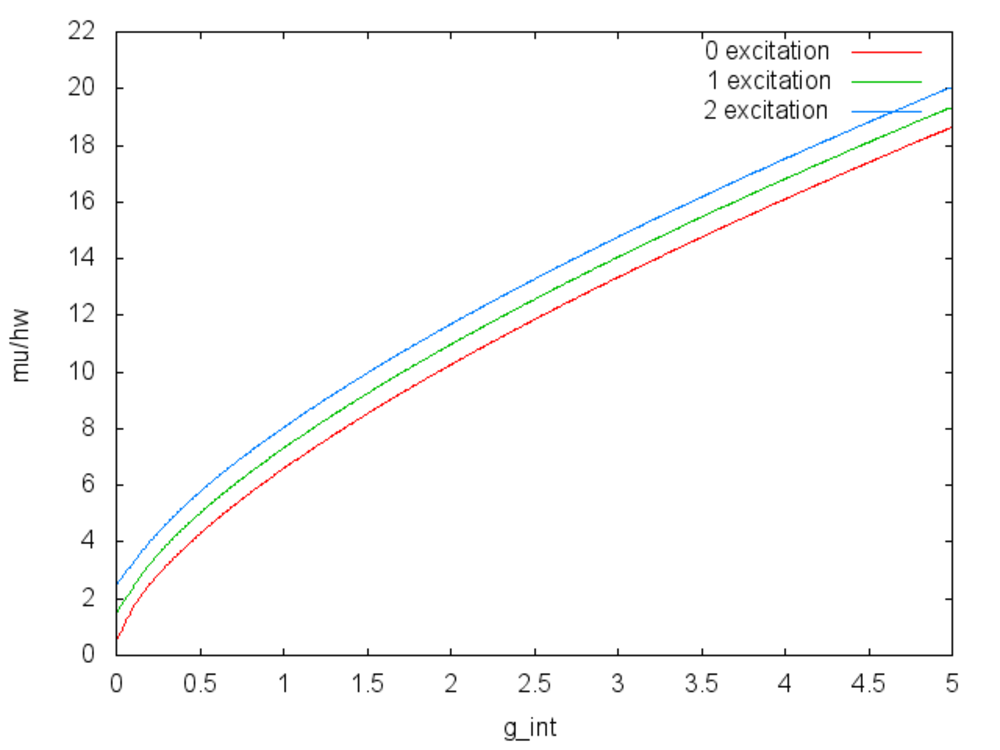
\includegraphics[width=0.9\linewidth]{cont_lin.pdf}
	\caption{Potencial qu\'imico para diferentes estados en su evoluci\'on en la no-linealidad}
	\label{Fig:cont_lin}
\end{figure}

\subsection{Solit\'on oscuro bajo un potencial arm\'onico}
Ahora veremos el comportamiento de estos defectos topol\'ogicos bajo un potencial arm\'onico. Como hemos visto estos objetos se comportan como una part\'icula con una masa asociada (negativa), aqu\'i comprobaremos este hecho. En primer lugar presionamos el bot\'on \textit{Dark solitons study}. Introducimos la posici\'on inicial del solit\'on, el n\'umero de oscilaciones que queremos que de e introduciremos en \textit{Number of symmetric solitons = 1}. Presionamos ahora el bot\'on \textit{START} y esperamos a que finalice el tiempo de computaci\'on. Ahora podemos entrar en el apartado \textit{MINUS}, en el vemos una gr\'afica donde se representa nuestro condensado para diferentes instantes de tiempo. En el podemos extraer el periodo de oscilaci\'on de nuestro solit\'on y con el podr\'iamos extraer su masa asociada. En el apartado \textit{PHASE} podemos comprobar que un solit\'on es un defecto topol\'ogico. En esta gr\'afica se representa la diferencia de fase entre la parte derecha del solit\'on y la parte izquierda, como se ha mencionado en teor\'ia, se introduce un cambio de fase $\pi$ pero como el solit\'on al oscilar adquiere velocidad este ya no introduce un 0 en la densidad, por lo tanto este cambio de fase es menor. Por \'ultimo podemos entrar en la evoluci\'on del estado y veremos como el solit\'on oscila con el tiempo.

\subsection{Interacci\'on entre dos solitones oscuros bajo un potencial arm\'onico}
 Como ya se ha mencionado, la interacci\'on entre dos solitones es repulsiva, ahora comprobaremos esta interacci\'on en presencia de un potencial arm\'onico. Para observar este fen\'omeno introducimos los mismos par\'ametros que en el apartado anterior pero ahora, seleccionaremos \textit{Number of symmetric solitons = 2}. Lo que calcularemos ahora es una soluci\'on con dos solitones impresos de forma sim\'etrica. Primero ejecutamos el programa con una posici\'on entre ellos mayor a 2. Podemos comprobar en el apartado \textit{MINUS} como el periodo es exactamente el mismo que con solo un solit\'on. Ha medida que hagamos los c\'alculos con una posici\'on mas pequeña entre ellos, veremos como el periodo se va reduciendo. A una poisici\'on muy pequeña veremos un r\'egimen totalmente repulsivo entre los solitones (recuperamos la interacci\'on para un background homogéneo). Podemos encontrar un estado ligado entre estos donde tendríamos una soluci\'on estacionaria con los solitones, como la que vemos en la Fig.~\ref{Fig:stati_3}. Es interesante recoger diversos valores del periodo para diferentes posiciones de los solitones, obtendr\'iamos una gr\'afica como la que se muestra en la Fig.~\ref{Fig:per}. No podemos recuperar con esta simulaci\'on un fuerte resultado (podr\'iamos pero el m\'etodo ser\'ia extensamente largo), que es que la energ\'ia de interacci\'on entre dos solitones es muy similar al potencial tipo part\'icula.
 
  \begin{figure}[tb]
 	\centering
 	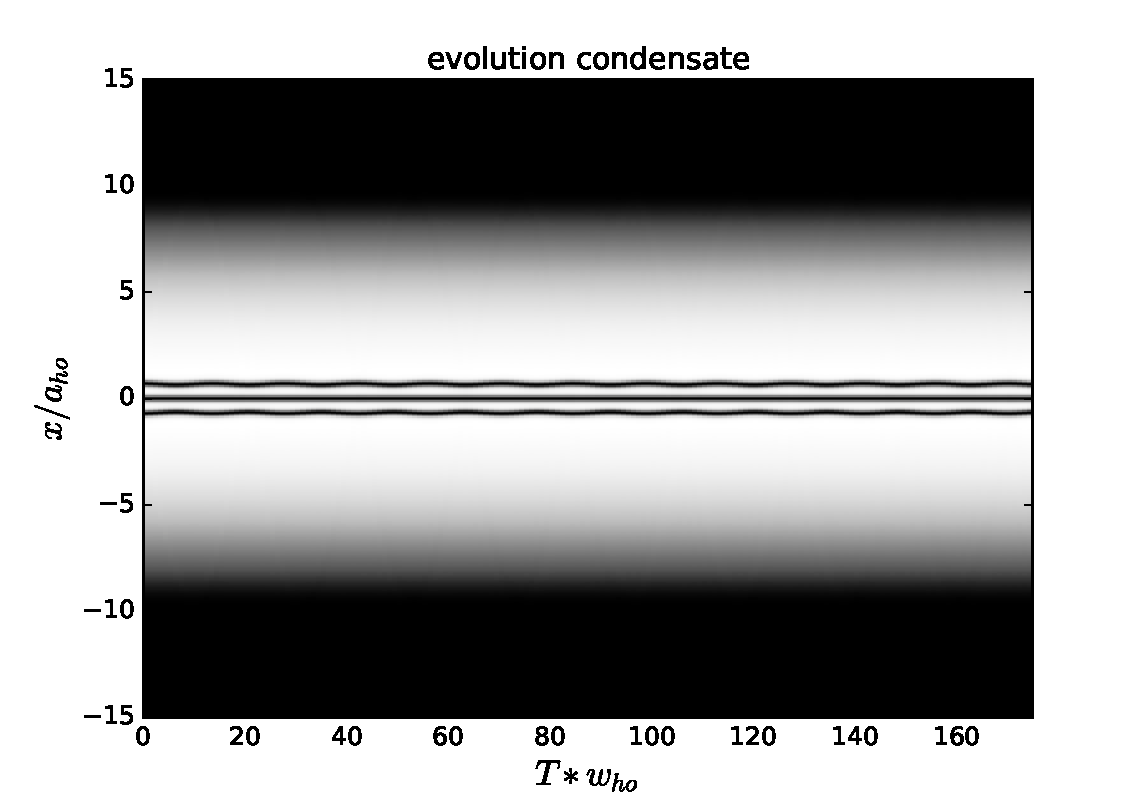
\includegraphics[width=0.9\linewidth]{stati_3.pdf}
 	\caption{Estado ligado para 3 solitones oscuros.}
 	\label{Fig:stati_3}
 \end{figure}
 
 \begin{figure}[tb]
 	\centering
 	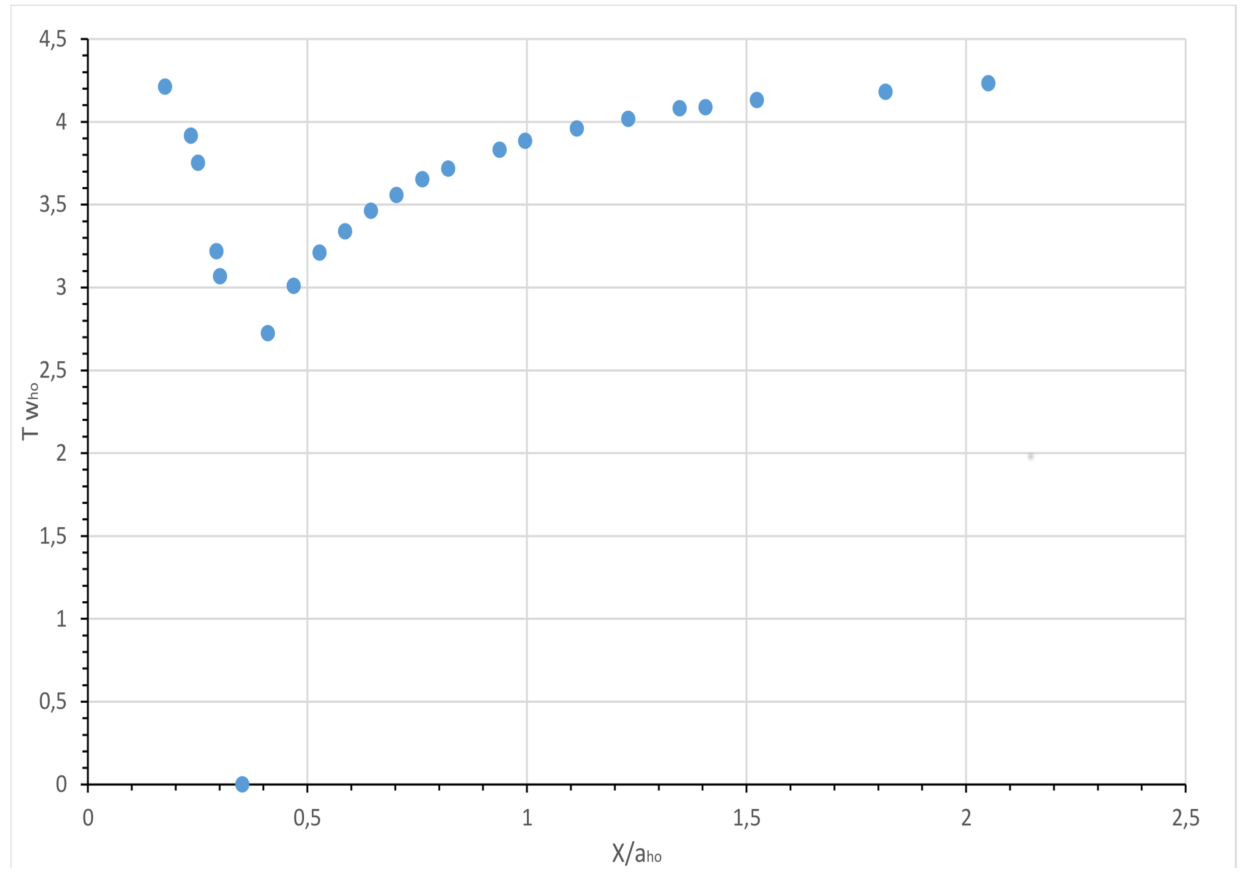
\includegraphics[width=0.9\linewidth]{periodo.pdf}
 	\caption{Evoluci\'on del periodo de dos solitones para diferentes posiciones sim\'etricas de estos}
 	\label{Fig:per}
 \end{figure}

\subsection{P\'endulo de Newton con solitones}
Ahora que hemos estudiado diferentes propiedades de los solitones oscuros y la condensaci\'on de Bose-Einstein, vamos a proceder con un ejemplo bastante interesante donde mezclaremos diversos conceptos utilizados.

Para inicializar este proceso debemos clicar en el m\'odulo \textit{Newton's cradle}, en \textit{Computation control} se nos abrir\'an diferentes comandos a controlar. B\'asicamente controlaremos dos estados, uno ser\'a el estado central sim\'etrico al que llamaremos la cadena de solitones; el otro ser\'a un estado que chocar\'a con el anterior, que ser\'a el estado inicialmente en movimiento. En \textit{number of solitons in motion} podemos controlar el n\'umero de solitones que queremos en el estado en movimiento (de 1 a 2). En \textit{initial position of solitons in motion} controlamos la posici\'on inicial de este mismo estado. Con \textit{number of oscilations} controlamos el tiempo total que durar\'a la simulaci\'on, b\'asicamente est\'a escalado con el periodo que tiene un \'unico solit\'on. Finalmente con \textit{number of solitons in chair} controlamos el estado central sim\'etrico estacionario, podemos seleccionar de cu\'antos solitones est\'a formado (de 1 a 3). Una vez est\'en todas las configuraciones seleccionadas iniciamos la simulaci\'on. 

En este m\'odulo nos interesaremos en la evoluci\'on del estado y en la gr\'afica \textit{MINUS}, donde podemos obtener gr\'aficas como la mostrada en la Fig.~\ref{Fig:new_crand}. Podemos observar un claro s\'imil con un fen\'omeno del mundo cl\'asico, el p\'endulo de Newton. No olvidemos que lo que tenemos aqu\'i es un condensado de Bose-Einstein y solitones oscuros. Sin embargo podemos ver que el comportamiento de estos es muy parecido al que tendr\'ian unas bolas con un volumen y masa bajo un potencial. 

\begin{figure}[tb]
	\centering
	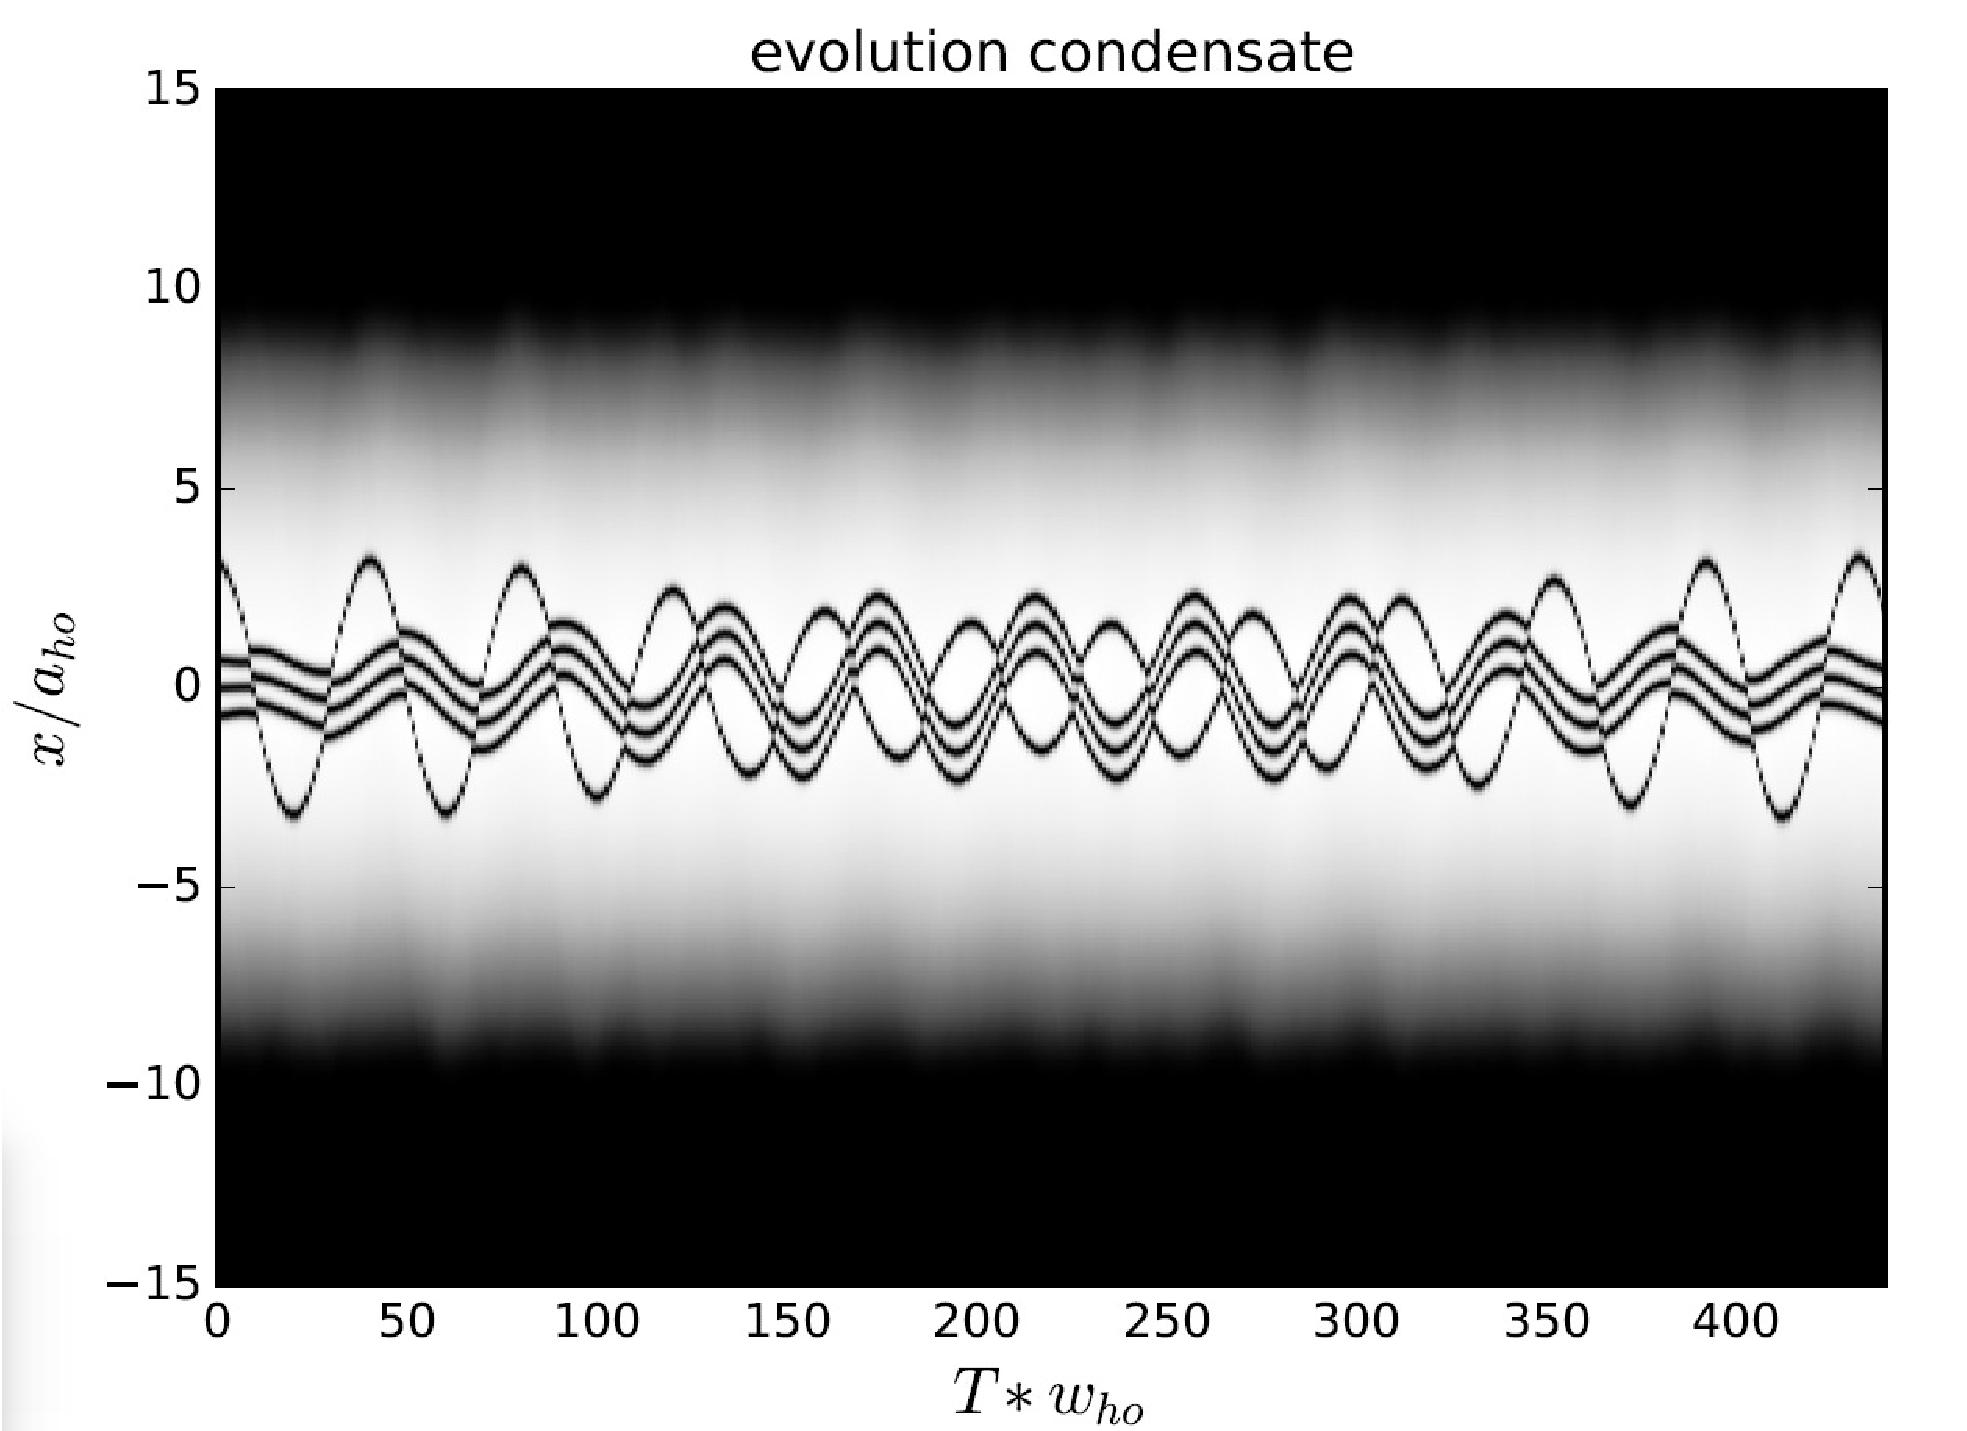
\includegraphics[width=0.9\linewidth]{new_crand.pdf}
	\caption{Evoluci\'on de un estado donde podemos observar el efecto del P\'endulo de Newton}
	\label{Fig:new_crand}
\end{figure}

\end{document}
